% 2021 全国乙卷理科第 18 题：四棱锥 P-ABCD，底面 ABCD 为矩形；逻辑图名 2021-national-b-science-t18-pyramid
% 隐藏棱 AD、DC、PD 以虚线表示；M 为 BC 中点，连结 PM。
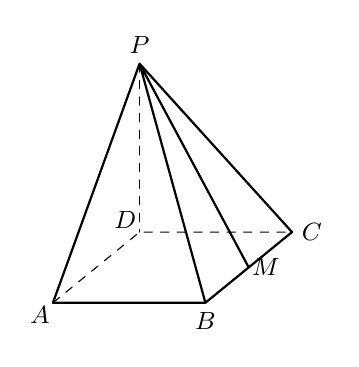
\begin{tikzpicture}[x=0.88cm,y=0.88cm,line cap=round,line join=round,font=\small]
  \coordinate (A) at (0,0);
  \coordinate (B) at (2.2,0);
  \coordinate (C) at (3.45,1.02);
  \coordinate (D) at (1.25,1.02);
  \coordinate (P) at (1.25,3.45);
  \coordinate (M) at (2.825,0.51);

  % Visible base and lateral edges
  \draw[thick] (A) -- (B) -- (C);
  \draw[thick] (P) -- (A) (P) -- (B) (P) -- (C) (P) -- (M);

  % Hidden rear edges
  \draw[dashed] (A) -- (D) -- (C);
  \draw[dashed] (P) -- (D);

  \node[above] at (P) {$P$};
  \node[below left,inner sep=1pt] at (A) {$A$};
  \node[below] at (B) {$B$};
  \node[right] at (C) {$C$};
  \node[above left,inner sep=1pt] at (D) {$D$};
  \node[right,inner sep=1pt] at (M) {$M$};
\end{tikzpicture}
